\chapter{Matrix Decompositions}

\section{SVD}

We have seen that hermitian matrices are always diagonalizable. What about general rectangular matrices?
The following theorem shows that one can always find two matrix $\bold{U}$ and $\bold{V}$
so that the matrix $\bold{U}^H\bold{A}\bold{V}$ will be diagonal. This can be written as 
$\bold{U}^H\bold{A}\bold{V} = \bold{\Sigma }$ or equivalently, $\bold{A} = \bold{U}\bold{\Sigma }\bold{V}^H$.

\begin{figure}[htbp]
    \centering
    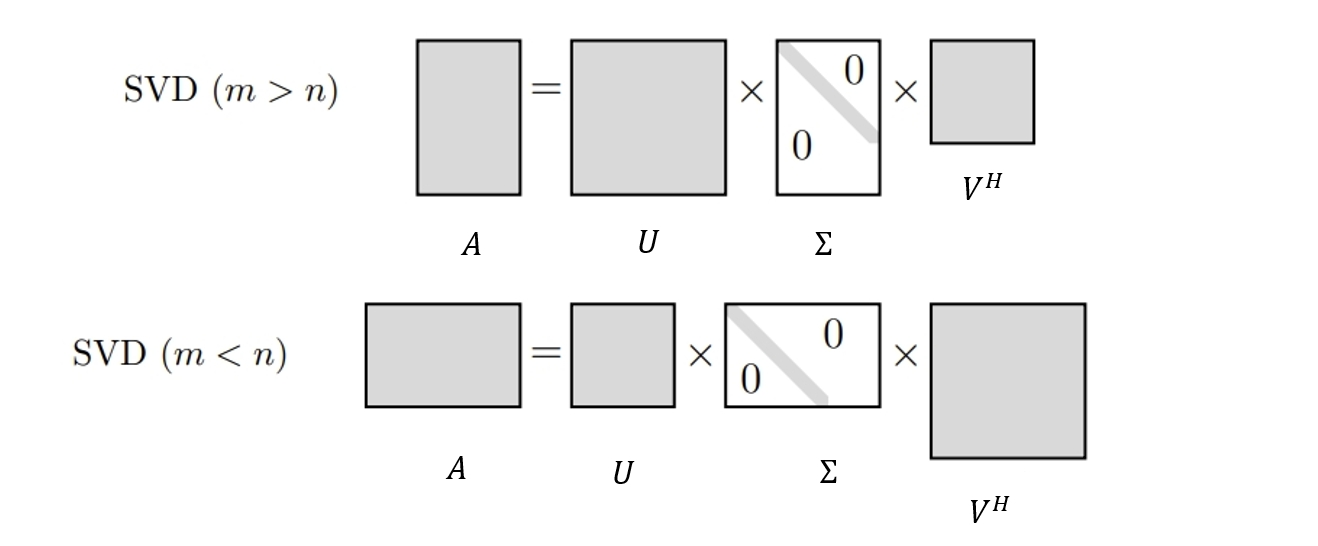
\includegraphics[width=0.6\textwidth]{figure/svd1.png}
    \caption{}
\end{figure}

\begin{remark}
    $\Sigma\in\C^{m\times n}$ is said to be diagonal if $\Sigma_{ij}=0$ for $i\neq j$.
    It has exactly $p=\min \{m,n\}$ diagonal entries and can be denoted by $\Sigma=\text{diag}\{d_1,...d_p\}$.
\end{remark}


\subsection{Singular value decomposition (SVD)}

\begin{theorem}{}{}
    Let $\bold{A}\in \C^{m\times n}$ and denote $p=\min\{m,n\}$.
    Denote the rank of $\bold{A}$ by $r$ ($0\leqs r\leqs p$).
    Then there are unitary matrices $\bold{U}\in \C^{m\times m}$ and $\bold{V}\in \C^{n\times n}$
    and a real diagonal matrix $\Sigma =\text{diag} \{\sigma_1,...,\sigma_p\}\in \R^{m\times n}$ such that 
    \begin{align*}
        \bold{A}=\bold{U}\bold{\Sigma}\bold{V}^H
    \end{align*}
    and 
    \begin{align*}
        \sigma_1\geqs ...\geqs \sigma_r\geqs \sigma_{r+1}=...=\sigma_p=0,
    \end{align*}
    the matrix $\Sigma$ is uniquely determined by $\bold{A}$.
\end{theorem}

\begin{proof}
    Let $\bold{C}=\bold{A}^H\bold{A}\in \C^{n\times n}$. Then $\bold{C}$ is square, hermitian, and positive semidefinite.
    Therefore, $\bold{C}=\bold{V}\Lambda\bold{V}$ for an unitary $\bold{V}\in \C^{n\times n}$
    and diagonal $\Lambda=\text{diag} \{\lambda_1,...\lambda_n\}$ with $\lambda_1\geqs ...\geqs \lambda_r>0=\lambda_{r+1}=...=\lambda_n$.
    
\end{proof}

\section{Reference}

\begin{itemize}
    \item \href{http://users.ece.northwestern.edu/~mya671/files/Matrix_YM_.pdf}{Matrix Decomposition}
    \item \href{https://math.berkeley.edu/~hutching/teach/54-2017/svd-notes.pdf}{SVD notes}
    \item \href{https://www.sjsu.edu/faculty/guangliang.chen/Math253S20.html}{Mathematical Methods for Data Visualization}
    \item \href{https://kuidu.github.io/nla/nla02.pdf}{SVD notes XMUT}
    \item \href{https://people.cas.uab.edu/~mosya/teaching/660new3.pdf}{Singular Value Decomposition}
\end{itemize}